\documentclass[12pt]{article}

\usepackage{fullpage}
\usepackage{graphicx, rotating, booktabs} 
\usepackage{times} 
\usepackage{natbib} 
\usepackage{indentfirst} 
\usepackage{setspace}
\usepackage{grffile} 
\usepackage{hyperref}
\usepackage{adjustbox}
\setcitestyle{aysep{}}


\singlespace
\title{\textbf{Appendix: Alliance Participation, Treaty Depth, and Military Spending}}
%\author{Joshua Alley}
\date{}

\bibliographystyle{apsr}

\begin{document}

\maketitle 

\singlespace 

This online appendix provides more detail about the multilevel model and checks the results. 
I also briefly describe a single-level test of the depth hypothesis and assess other measures of alliance treaty depth. 


\section{Descriptive Statistics of Key Variables} 

This section provides two tables of descriptive statistics for the state and alliance-level variables. 


\begin{table}[!htbp] \centering 
  \caption{State-Level Variables} 
  \label{tab:state-level-sum} 
\begin{tabular}{@{\extracolsep{5pt}}lccccccc} 
\\[-1.8ex]\hline 
\hline \\[-1.8ex] 
Statistic & \multicolumn{1}{c}{N} & \multicolumn{1}{c}{Mean} & \multicolumn{1}{c}{St. Dev.} & \multicolumn{1}{c}{Min} & \multicolumn{1}{c}{Pctl(25)} & \multicolumn{1}{c}{Pctl(75)} & \multicolumn{1}{c}{Max} \\ 
\hline \\[-1.8ex] 
International War & 8,280 & 0.029 & 0.167 & 0 & 0 & 0 & 1 \\ 
Civil War Participant & 8,280 & 0.082 & 0.275 & 0 & 0 & 0 & 1 \\ 
Rival Military Spending & 8,280 & $-$0.062 & 0.432 & $-$0.263 & $-$0.263 & 0.101 & 3.444 \\ 
GDP growth & 8,280 & 0.008 & 0.516 & $-$3.699 & $-$0.187 & 0.184 & 20.202 \\ 
POLITY & 8,280 & $-$0.011 & 0.502 & $-$0.738 & $-$0.532 & 0.496 & 0.633 \\ 
Cold War & 8,280 & 0.503 & 0.500 & 0 & 0 & 1 & 1 \\ 
Annual MIDS & 8,280 & $-$0.060 & 0.384 & $-$0.245 & $-$0.245 & 0.144 & 9.869 \\ 
\hline \\[-1.8ex] 
\end{tabular} 
\end{table} 



\begin{table}[!htbp] \centering 
  \caption{Alliance-Level Variables. Number of members, foreign policy disagreement, average democracy, and average threat are all measured for the first year of the alliance.} 
  \label{tab:all-level-sum} 
\begin{tabular}{@{\extracolsep{5pt}}lccccccc} 
\\[-1.8ex]\hline 
\hline \\[-1.8ex] 
Statistic & \multicolumn{1}{c}{N} & \multicolumn{1}{c}{Mean} & \multicolumn{1}{c}{St. Dev.} & \multicolumn{1}{c}{Min} & \multicolumn{1}{c}{Pctl(25)} & \multicolumn{1}{c}{Pctl(75)} & \multicolumn{1}{c}{Max} \\ 
\hline \\[-1.8ex] 
Latent Depth Mean & 190 & 0.069 & 0.898 & $-$0.843 & $-$0.776 & 0.878 & 1.979 \\ 
Unconditional Military Support & 190 & 0.521 & 0.501 & 0 & 0 & 1 & 1 \\ 
Economic Issue Linkages & 190 & 0.579 & 0.495 & 0 & 0 & 1 & 1 \\ 
Foreign Policy Concessions & 190 & 0.805 & 0.860 & 0 & 0 & 1 & 3 \\ 
Number of Members& 190 & 3.879 & 5.677 & 2 & 2 & 3 & 43 \\ 
Foreign Policy Disagreement & 190 & 0.653 & 0.346 & $-$0.103 & 0.360 & 0.972 & 1.000 \\ 
Average Democracy & 190 & $-$2.127 & 5.708 & $-$10 & $-$7 & 1.5 & 10 \\ 
Wartime Alliance & 190 & 0.126 & 0.333 & 0 & 0 & 0 & 1 \\ 
Asymmetric Obligations & 190 & 0.216 & 0.412 & 0 & 0 & 0 & 1 \\ 
Average Threat & 190 & 0.356 & 0.163 & 0.000 & 0.253 & 0.473 & 0.674 \\ 
US Membership & 190 & 0.095 & 0.294 & 0 & 0 & 0 & 1 \\ 
USSR Membership & 190 & 0.074 & 0.262 & 0 & 0 & 0 & 1 \\ 
\hline \\[-1.8ex] 
\end{tabular} 
\end{table} 



\section{Priors}

\autoref{tab:priors} summarizes the prior distributions in the multilevel model. 
All priors are weakly informative relative to the scale of the data. 
$\nu$ is the degrees of freedom for the t-distribution, and the gamma prior is the recommended prior for STAN \citep{JuarezSteele2010}. 

\begin{table} % Create a table of priors.
\begin{center}
\begin{tabular}{c} 
$ p(\alpha) \sim N(0, 1)$  \\
$ p(\sigma) \sim \mbox{half-}N(0, 1) $ \\
$ p(\alpha^{yr}) \sim N(0, \sigma^{yr}) $ \\ 
$ p(\sigma^{yr}) \sim N(0, 1) $ \\
$ p(\alpha^{st}) \sim N(0, \sigma^{st}) $ \\ 
$ p(\sigma^{st}) \sim \mbox{half-}N(0, .5) $ \\ 
$ p(\sigma^{all}) \sim \mbox{half-}N(0, .5) $ \\
$ p(\beta) \sim N(0, .5) $ \\
$ p(\gamma) \sim N(0, .5) $ \\ 
$ p(\nu) \sim Gamma(2, 0.1)$ 
\end{tabular} 
\caption{Summary of Priors in Multilevel Model} 
\label{tab:priors}
\end{center} 
\end{table} 


\section{Hamiltonian Monte Carlo Diagnostics}

There were no divergent iterations in either sample running 4 chains for 2,000 iterations with 1,000 warmup iterations. 
The $\hat{R}$ is less than 1.1 for all parameters in both samples. 
Trace plots in \autoref{fig:trace-all-min} indicate good mixing of the chains for the alliance-level parameters. 
Taken together, all of this implies that the chains adequately explored the posterior distribution. 

\begin{figure}[htbp]
	\centering
		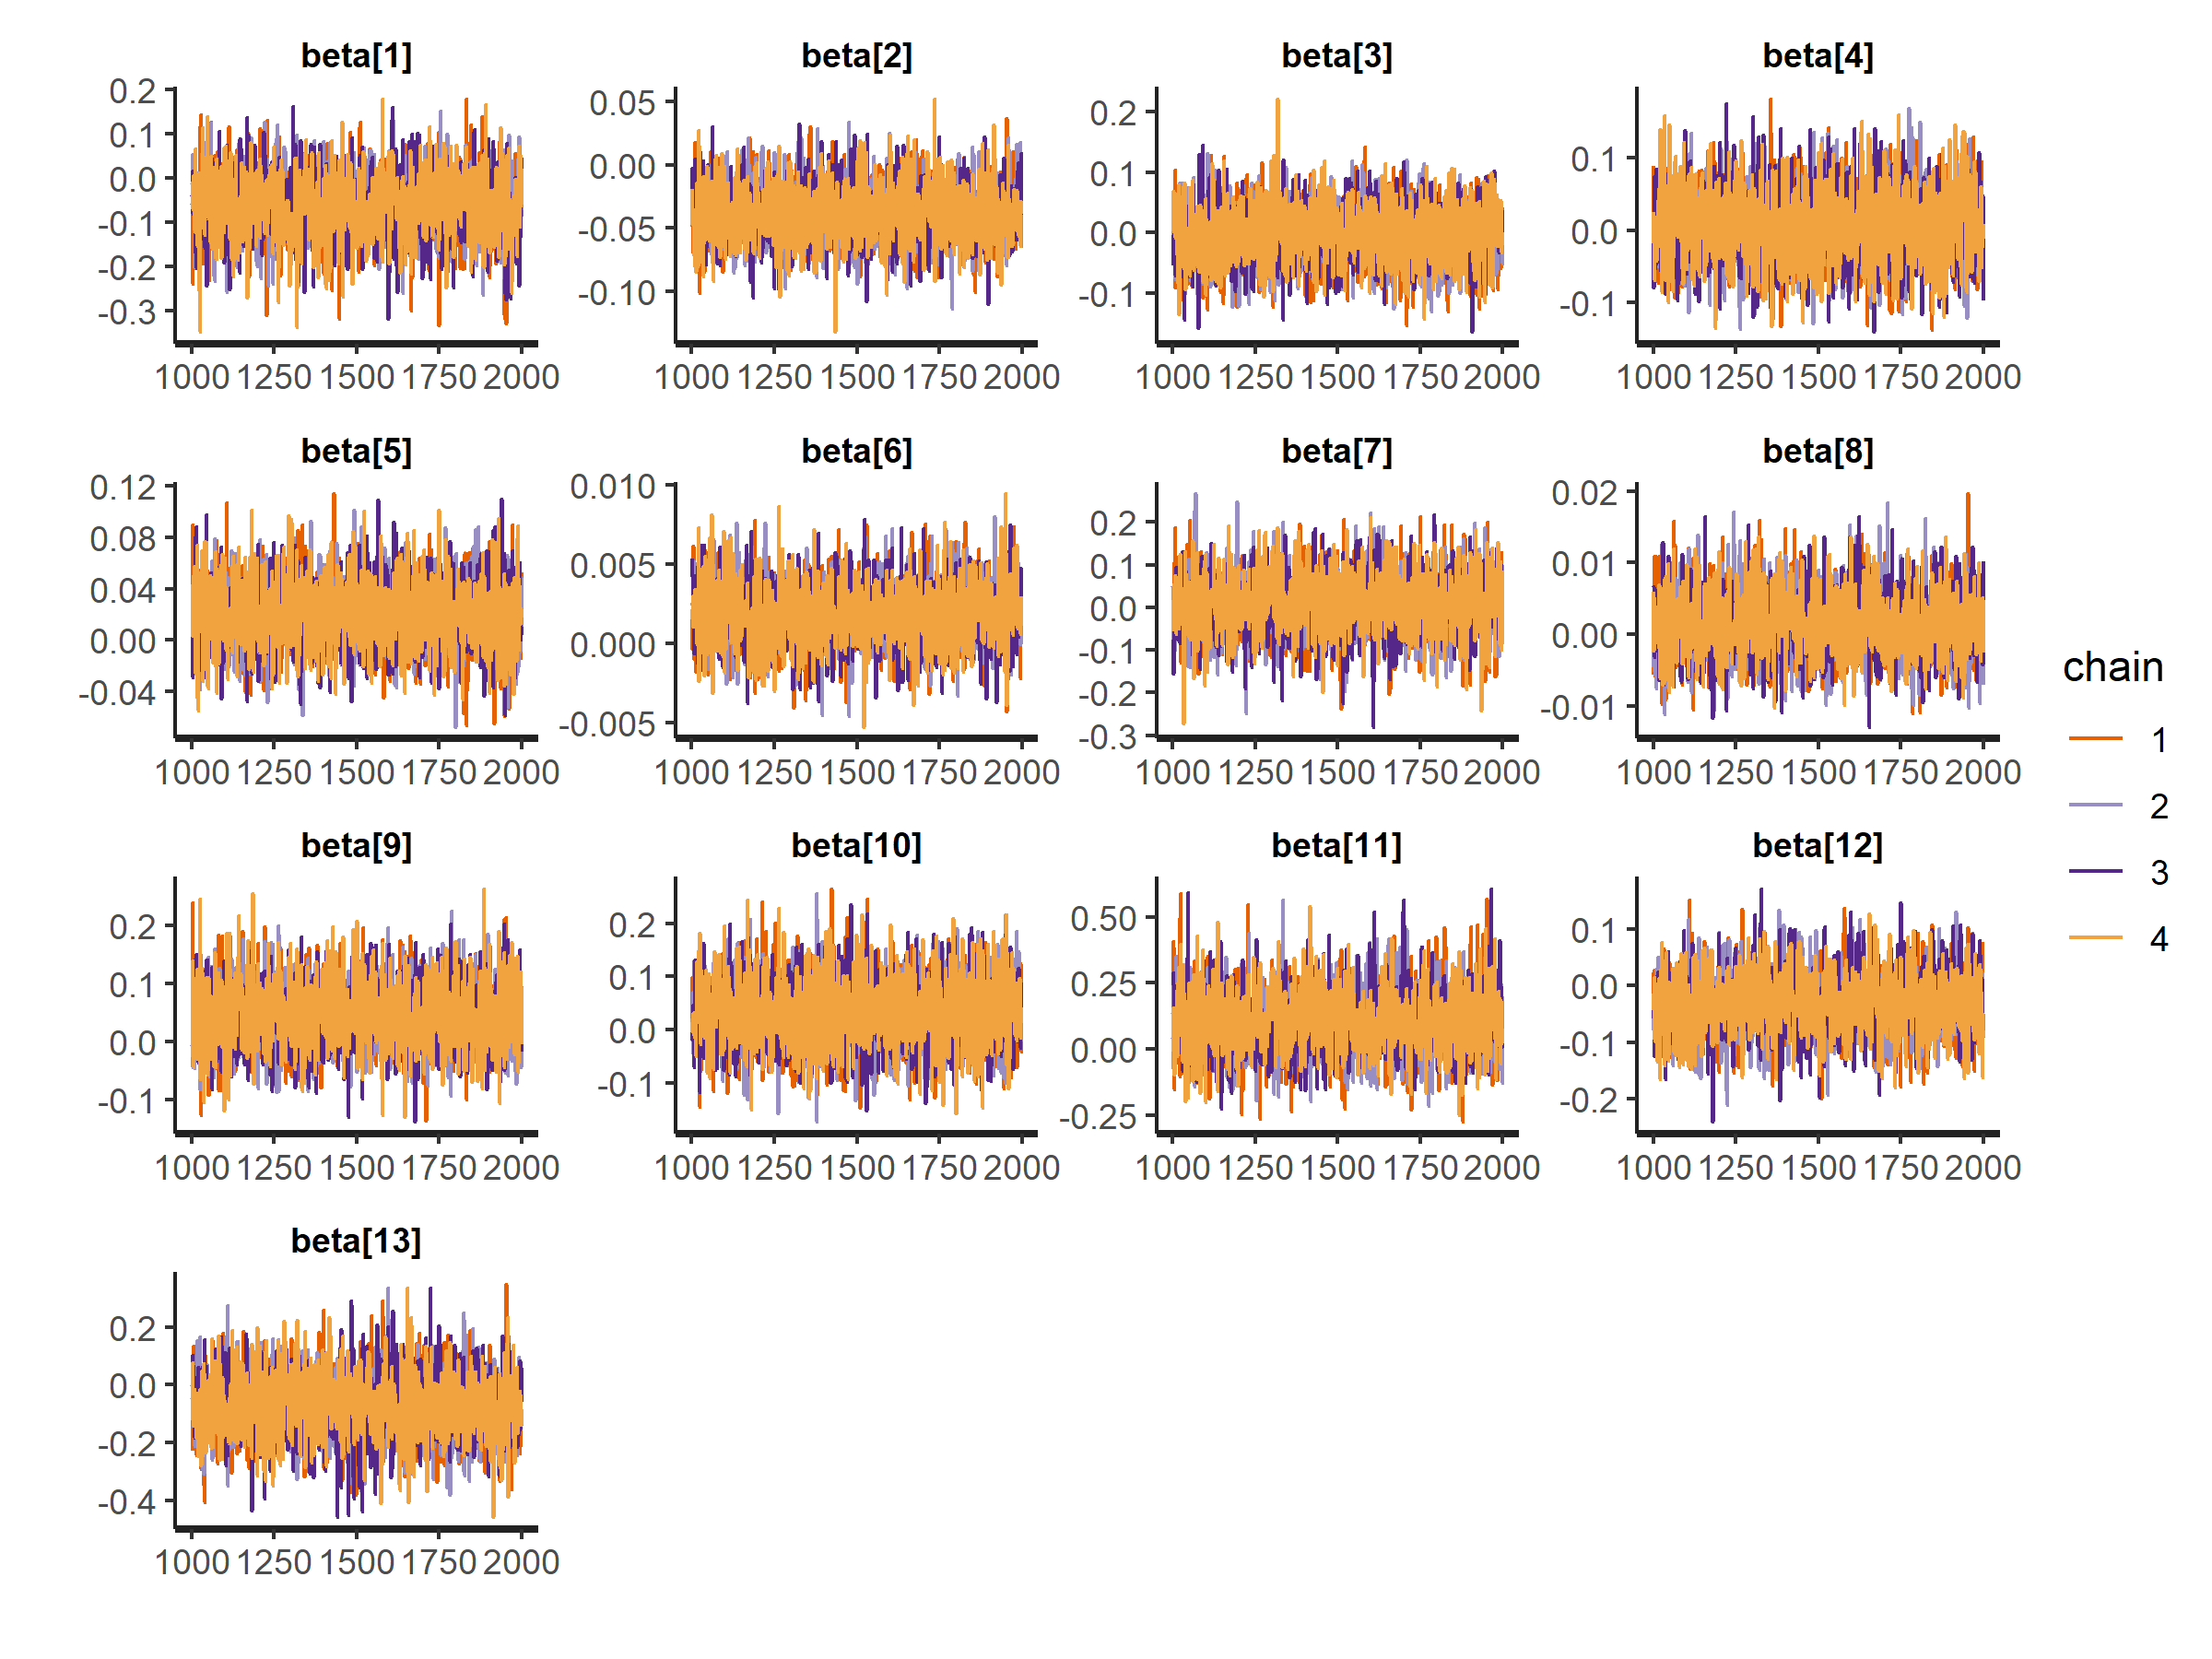
\includegraphics[width=0.95\textwidth]{trace-all-min.png}
	\caption{Traceplot of alliance level parameters in the non-major power sample.}
	\label{fig:trace-all-min}
\end{figure}



%\section{Normalizing Allied Capability}
%
%% Justify use of annual normalization
%As noted in the paper, I place allied capability in the membership matrix \textbf{Z} on the same scale as the other parameters by normalizing it by year. 
%Within each year, I divide the total military spending of allied states by the maximum value, so capability values within each year range from just above zero to one. 
%This ensures that allied capability is comparable within years, and that I do not treat more modern alliances as the most capable due to increases in raw defense budget sizes. 
%
%
%The choice of this specific normalization is less theoretically informed than using capability itself. 
%Therefore, I assessed the use of different normalizations and rescalings for allied capability by comparing model fit. 
%I fit three models in addition to the one presented in the paper. 
%The first rescaled allied capability by dividing each capability value by the maximum of capability without grouping alliances by year. 
%The second rescaled alliance capability by dividing by two standard deviations, which is problematic because it introduces negative capability values. 
%The last used total allied CINC scores instead of military spending as an indicator of allied capability, which also facilitates comparisons of allied capability within years. 
%CINC scores measure the share of total world military capability each state has in a particular year, so it is useful for comparing allied capability within years \citep{SingerCINC1988}. 
%
%
%After estimating these three models, I used leave-one-out (LOO) cross validation to assess model fit \citep{Vehtarietal2017}. 
%LOO estimates pointwise out-of-sample prediction accuracy using the log-likelihood evaluated at the posterior simulations of the parameter values.\footnote{The widely applicable information criteria (WAIC) produces similar results, but the estimates for the CINC model may be driven by an unusual observation.} 
%All diagnostics indicate the LOO results are not driven by unusual observations. 
%As with other information criteria, lower values indicate better fit. 
%
% 
%
%\begin{table}[ht]
%\centering
%\begin{tabular}{rrrrrrrrr}
%  \hline
% Allied Capability & elpd\_diff & se\_diff & elpd\_loo & se\_elpd\_loo  \\ 
%  \hline
%  Normalized by Year & 0.000 & 0.000 & -1159.513 & 184.714 \\ 
%  Rescaled by Maximum & -3.165 & 2.643 & -1162.679 & 184.723  \\ 
%  Recaled by 2SD & -10.749 & 6.116 & -1170.262 & 184.741  \\ 
%  Total Allied CINC & -12.308 & 5.576 & -1171.821 & 184.683  \\ 
%   \hline
%\end{tabular}
%\caption{Leave-one-out cross validation to assess model fit with different rescalings or normalizations of alliance capability. }
%\label{tab:loo-zcontents}
%\end{table}
%
%\autoref{tab:loo-zcontents} summarizes the assessment of each model using the expected log pointwise predictive density (elpd). 
%I use the model from the paper as the comparison model: a negative elpd\_diff implies the normalized model fits the data better. 
%The difference also has some uncertainty, which is summarized by the se\_diff column of \autoref{tab:loo-zcontents}. 
%The other three models have a negative elpd\_diff compared to the model with normalized capability by year. 
%For the models with CINC and rescaling by two standard deviations the difference is large, relative to the se\_diff, so there is a clear preference for the normalized model. 
%Normalizing by year provides at best a marginal improvement over a model where capability is rescaled using the maximum. 
%Rescaling capability by the maximum produces similar inferences about alliance characteristics, including treaty depth. 



\section{Fake Data Simulation Check}


With any complicated model, simulating fake data and seeing if the model can recover known parameters is essential. 
Fake-data simulation helps validate results from observed data and identify problems. 
This section summarizes results from fitting the multilevel model to fake data.


I simulated a dataset of 2000 t-distributed observations with 50 states observed for 200 years and 100 alliances. 
The outcome has a different scale than the military spending outcome variable, so coefficient values here do not match the paper.  
I then simulated two state and alliance level variables and took a piece of the matrix of state membership in alliances. 
Last, I ran the model without evaluating the likelihood, generating a posterior prediction of the outcome based on the fake data.


To check whether the model could recover known parameters, I took the 12th draw of the posterior distribution.
This draw included a simulated outcome for each observation and a set of coefficients. 
I then fit the multilevel model on the simulated outcome values and checked whether the credible intervals contained the corresponding parameter values. 
If a parameter is within the 90\% credible interval, the model captures it. 


The model recovers known parameters with a high degree of accuracy. 
As shown by \autoref{fig:beta-sim-res}, the two credible intervals of the alliance-level regression include the known values.
Credible interval coverage for the variance hyperparameters and $\gamma$ parameters is also acceptable. 
\begin{figure}[htbp]
	\centering
		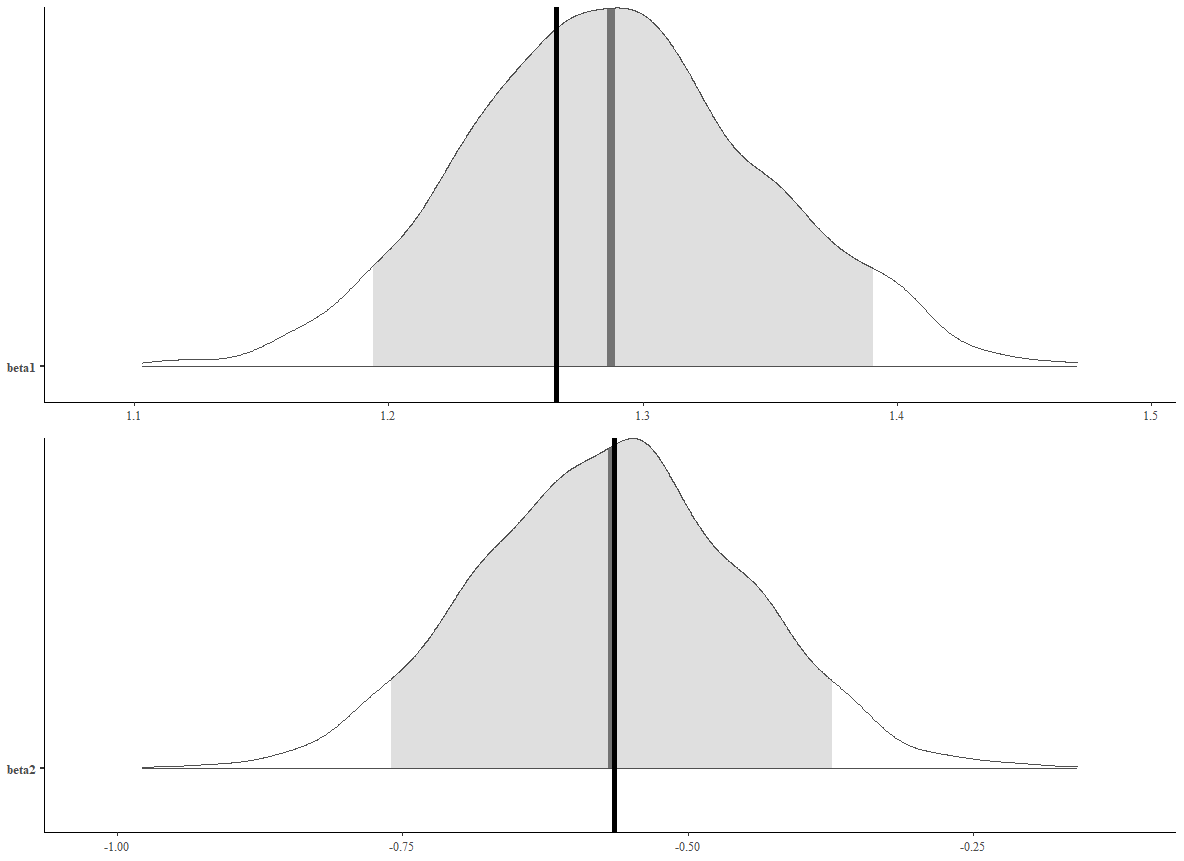
\includegraphics[width=0.95\textwidth]{beta-sim-res.png}
	\caption{Posterior distributions of $\beta$ parameters from fitting multilevel model to fake data. The black vertical line marks the known parameter value, and the grey area is the 90\% credible interval.}
	\label{fig:beta-sim-res}
\end{figure}


Even with small multiples, the 100 $\lambda$ parameters are hard to plot, so I offer a descriptive summary here. 
Among the $\lambda$ parameters, 93 of 100 intervals contain the known $\lambda$ value.
Given the large number of parameters and smaller sample, this is acceptable accuracy. 
Even the seven inaccurate confidence intervals were quite close--- all were within .015 of the known parameter.\footnote{Fine margins around these intervals implies that the exact number of accurate $\lambda$ intervals is sensitive to simulation variance.}



\section{Robustness Check: Alternative Measure of Military Spending}

The main findings in the manuscript rely on the Correlates of War military spending. 
Due to reporting issues, definition problems and measurement challenges, other measures of military spending could lead to different results. 
I check the robustness of my results by using \citet{Nordhausetal2012}'s measure of military spending, which combines data from the COW project and the Stockholm International Peace Research Institute (SIPRI). 
\citet{DigiuseppePoast2016} use this measure of military spending in their paper. 


I estimate the same multilevel model on this measure of military spending, which covers from 1949 to 2001. 
This model also checks whether how treaty depth modifies the impact of alliance participation on military spending changes after World War II.
Because the coefficient on a lagged dependent variable in this model is close to one, implying probable non-stationarity in levels, I use changes in military spending as the outcome of interest. 


\begin{figure}[htbp]
	\centering
		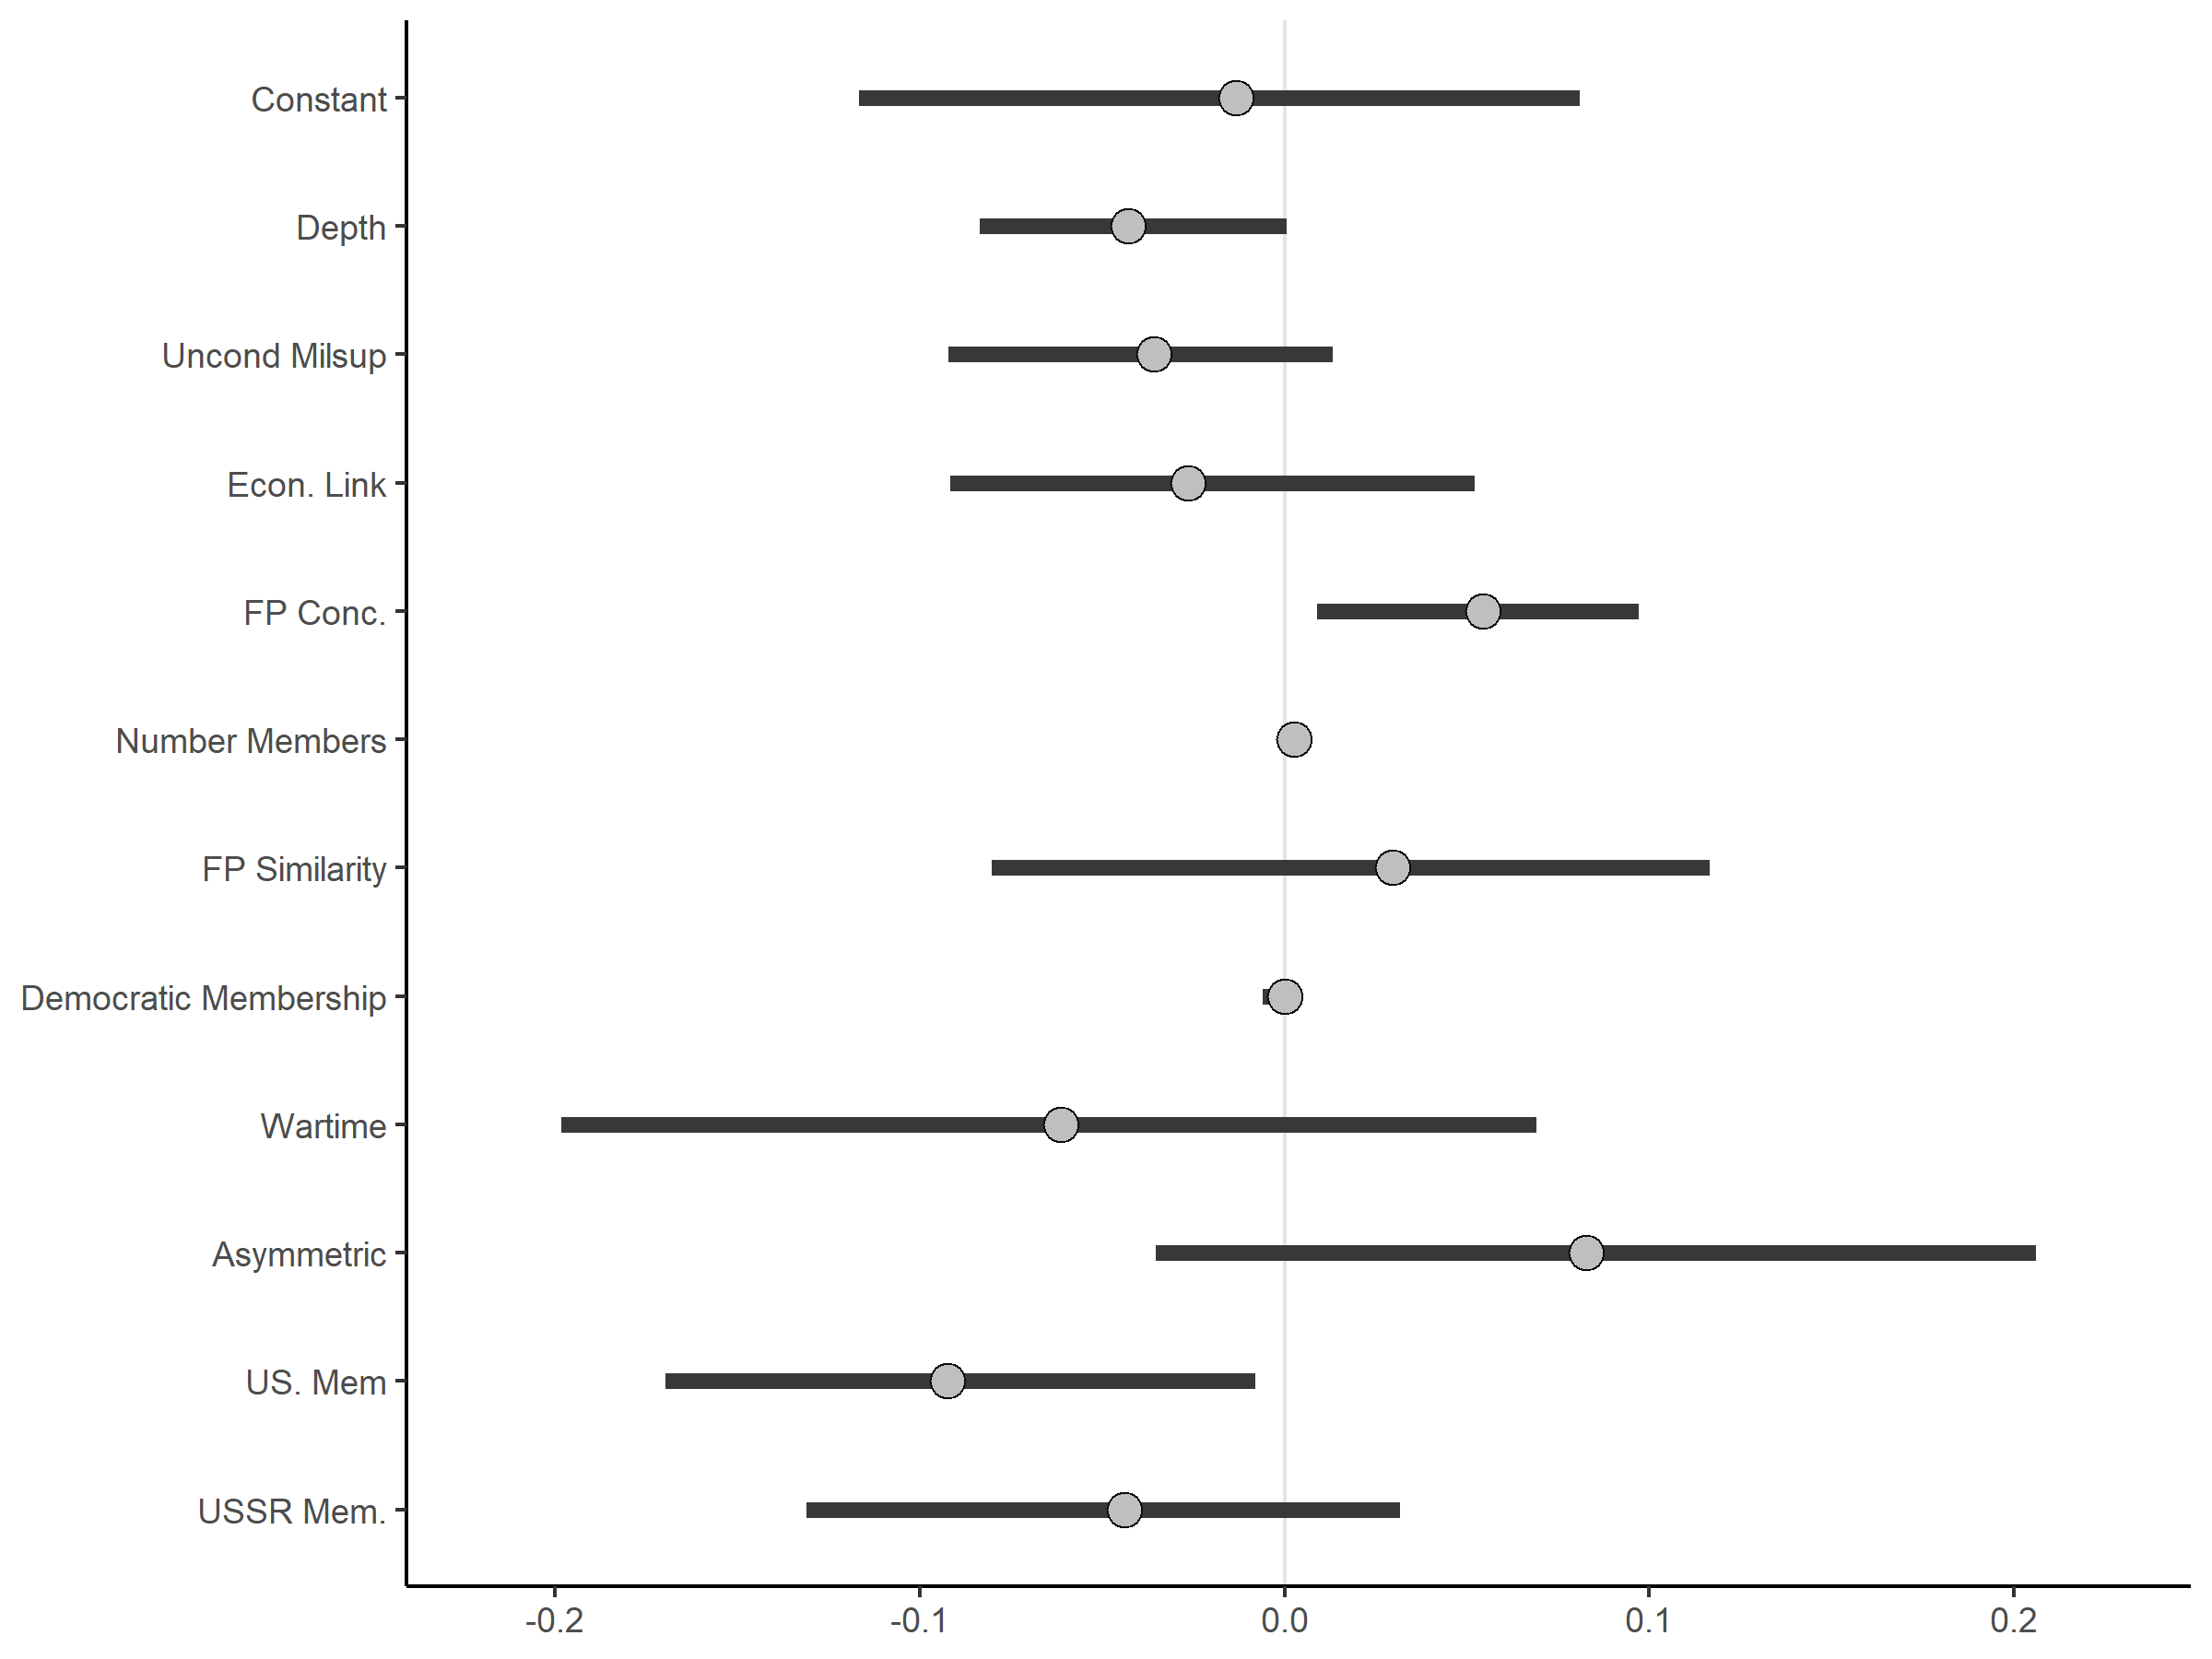
\includegraphics[width=0.95\textwidth]{post45-beta-res.png}
	\caption{90\% credible intervals of the $\beta$ parameters from an analysis of changes in non-major power military spending from 1949 to 2001.}
	\label{fig:post45-beta-res}
\end{figure}


\autoref{fig:post45-beta-res} summarizes the alliance-level regression parameters. 
As with the COW data, the credible interval for treaty depth is negative and does not overlap zero. 
All the parameter estimates are similar in this data, which increases my confidence that the results are not driven by the COW spending data. 

 


\section{Robustness Check: Single-Level Regression}


Though the multilevel model best reflects the theory, I also fit some more standard panel data models. 
In what follows, I briefly present results from robust regressions of state-year percentage changes in military spending in the same sample of non-major powers. 
As in the multilevel model, I applied the inverse hyperbolic sine transformation to the outcome. 
In these models, I employ two indicators of alliance depth. 
The first is the average depth of a state's alliances. 
The second is a dummy which equals 1 if a state has at least one alliance with greater than average depth. 
Both variables compare states with different depth in their alliance portfolio. 
In addition to the state-level controls in the multilevel model, I included average alliance size, average allied democracy and the log of total allied capability as controls. 


I estimated several models, including robust regressions on non-major powers and non-major powers in alliances. 
Comparing non-major powers with at least one alliance provides a crude approximation of the depth coefficient in the multilevel model, which compares deep and shallow alliances. 
I also applied state and year fixed effects to an OLS model of percentage changes in defense expenditures. 
The estimated association between average treaty depth and military spending changes is summarized in \autoref{fig:single-level-mplot}. 
Results are inconsistent- I do not reject the null hypothesis for the average depth measure unless the model includes state and year fixed effects. 
The deep alliance dummy coefficient estimate is negative and statistically significant across all samples and model specifications, however. 
The dummy variable is closest to \citet{DigiuseppePoast2016}'s design. 

\begin{figure}[htbp]
	\centering
		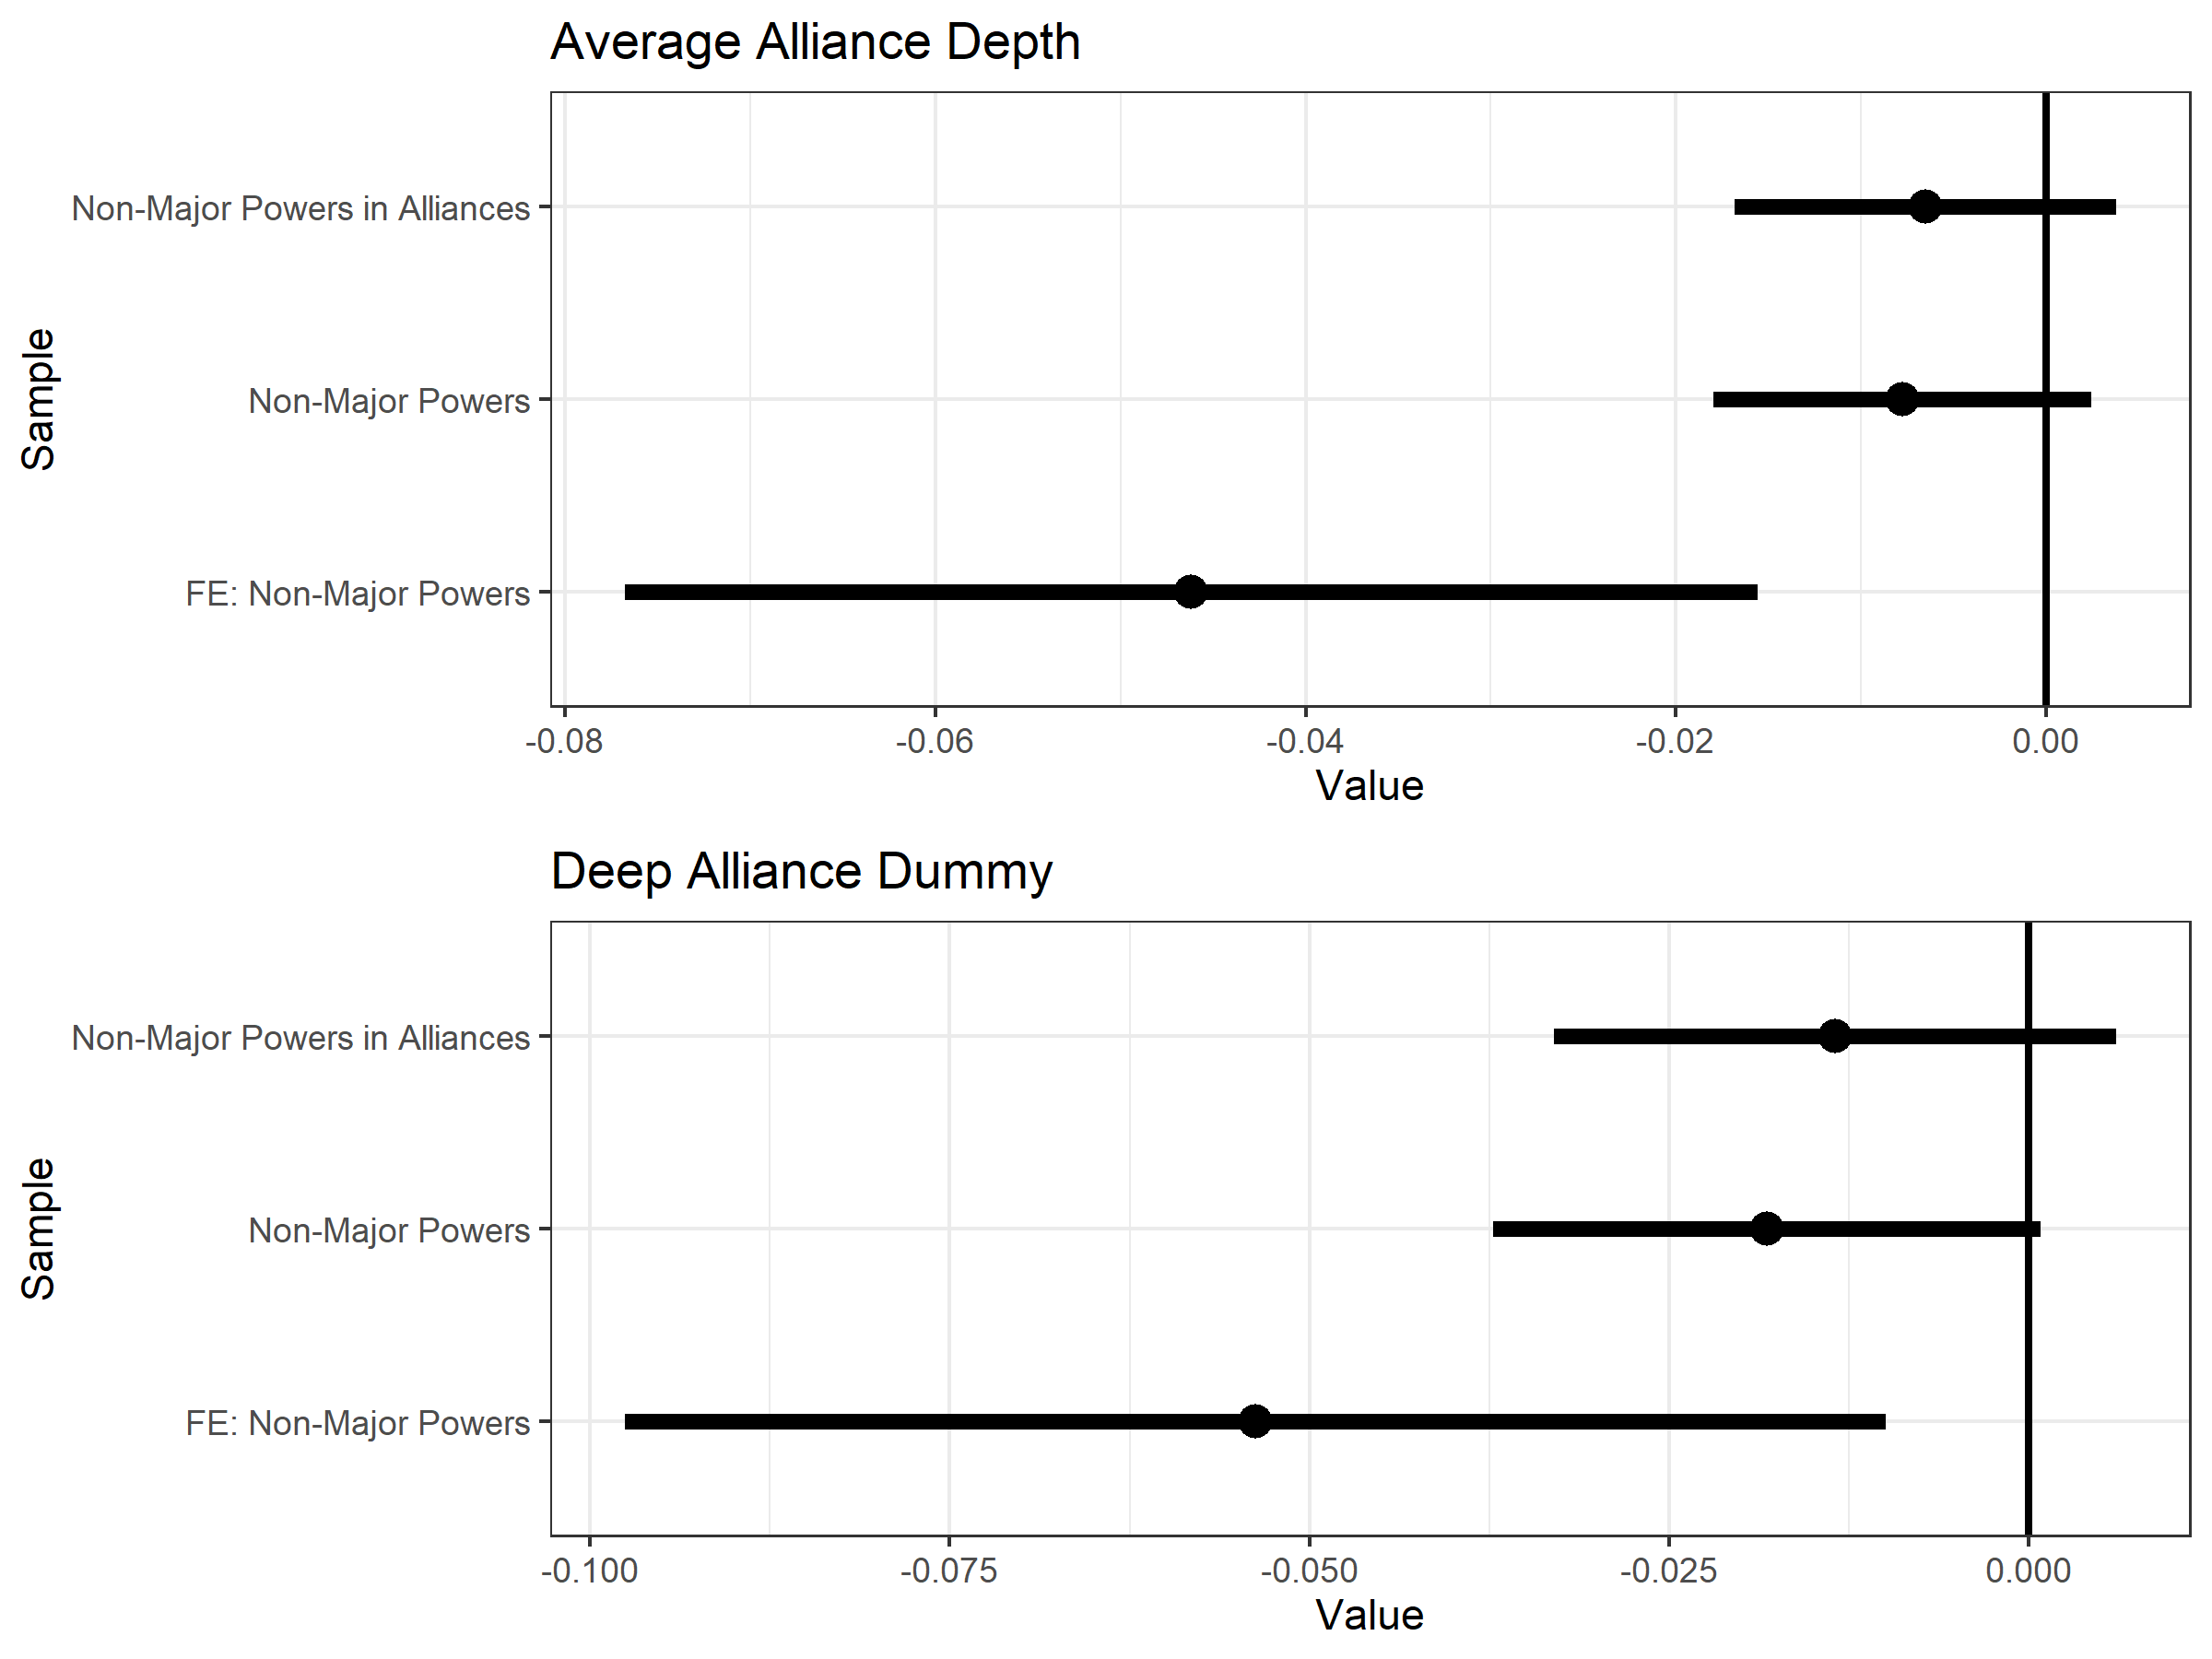
\includegraphics[width=0.95\textwidth]{single-level-mplot.png}
	\caption{Estimated effect of average alliance treaty depth or a dummy indicator of participation in a deep alliance on percentage changes in non-major power military spending from 1816 to 2007.}
	\label{fig:single-level-mplot}
\end{figure}

%
%I focus on the deep alliance dummy because the state-level averages may be misleading, and the deep alliance dummy matches \citet{DigiuseppePoast2016}'s design.
%To assess the robustness of the deep alliance dummy coefficient estimate in the sample of non-major powers, I performed Extreme Bounds analysis. 
%Specifically, I present results from \citet{Sala-i-Martin1997}'s method of bounds analysis in \autoref{fig:eba-single-level}. 
%This uses linear regression, so there is an imperfect comparison with the above robust regressions. 
%
%
%\autoref{fig:eba-single-level} shows the distribution of the deep alliance coefficient and an indicator of whether the alliance includes economic agreements. 
%Across many specifications, where all regression coefficients are doubtful, the CDF of the deep alliance coefficient has 90\% negative mass. 
%Even though the normality assumption is clearly violated, the histogram in \autoref{fig:eba-single-level} shows little evidence having a deep alliance increases percentage changes in military spending. 
%The bounds analysis indicates a deep alliance dummy is a robust predictor of percentage changes in military spending across over 1500 single-level model specifications. 
%
%
%\begin{figure}[htbp]
%	\centering
%		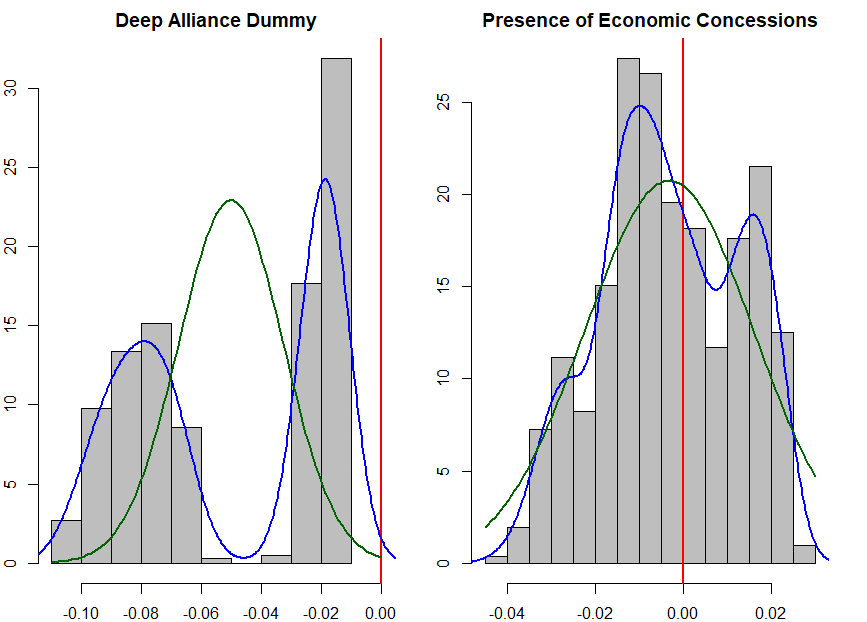
\includegraphics[width=0.95\textwidth]{eba-single-level.png}
%	\caption{Histogram of coefficient values for a deep alliance dummy and economic concessions in a single-level robust regression of non-major powers. Each dummy variable marks whether a state has at least one alliance with greater than average depth or economic concessions.}
%	\label{fig:eba-single-level}
%\end{figure}




\section{Alternative Measures of Alliance Treaty Depth}

This part of the appendix compares my latent measure of treaty depth with similar measures in earlier research.  
I first show that there are important differences between my measure and the military institutionalization measure of \citet{LeedsAnac2005}, but using military institutionalization instead of latent depth generates similar inferences about how treaty depth modifies the impact of alliance participation. 
Then I describe the conceptual and empirical differences between my latent measure and that of \citet{BensonClinton2016}.


\subsection{Leeds and Anac 2005}


\citet{LeedsAnac2005} create an ordinal measure of alliance treaty depth to study whether alliance institutionalization improves treaty reliability and performance in offensive and defense alliances. 
They argue that commitments of an integrated military command, common defense policy, or any basing rights generate high military institutionalization. 
Official contact between military officials, formal organizations, providing training or technology, subordination of forces, or specific contributions reflect moderate institutionalization. 
If at least one factor is present, Leeds and Anac assign alliance the highest corresponding level of institutionalization. 
This approach assumes that alliances with multiple sources of depth as just as deep/institutionalized as alliances with one factor and understates the amount of variation in alliance treaty depth. 


\begin{figure}[htbp]
	\centering
		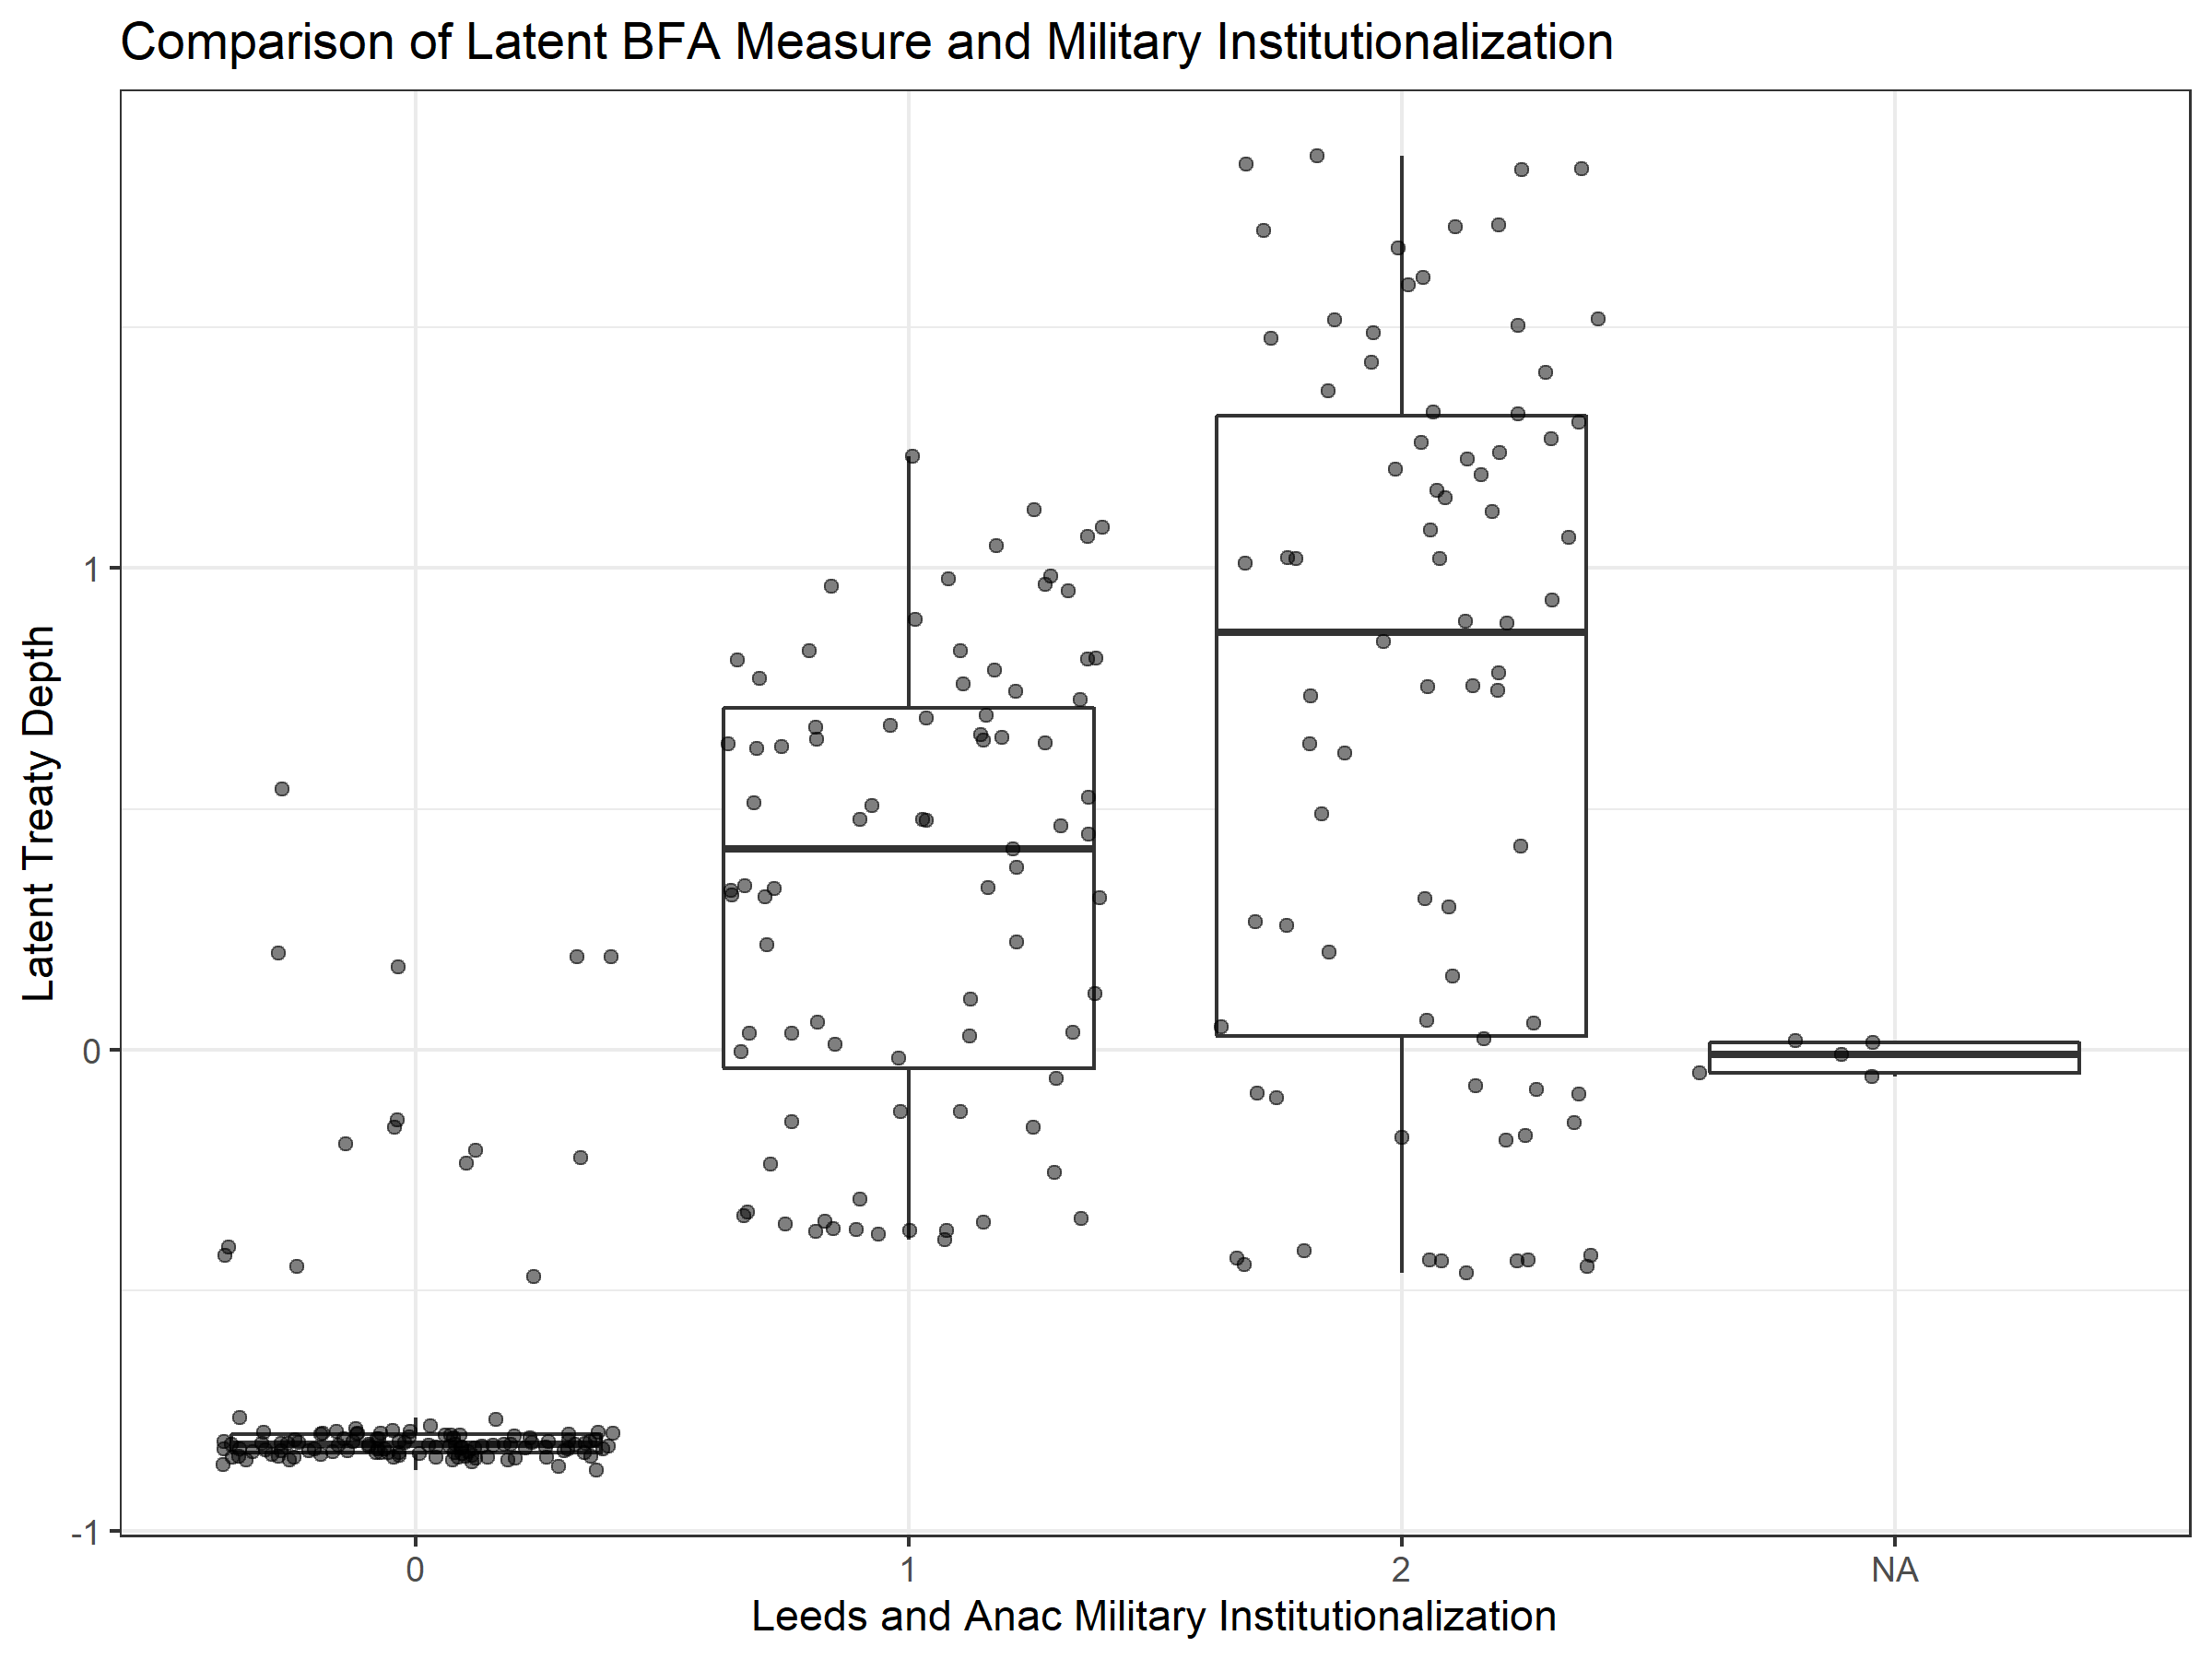
\includegraphics[width=0.95\textwidth]{leeds-anac-comp.png}
	\caption{Scatter plot of latent treaty depth across the values of military institutionalization from \citet{LeedsAnac2005}. The box plots summarize the distribution of latent treaty depth within each category of military institutionalization. Points are jittered within each level of the institutionalization score.}
	\label{fig:leeds-anac-comp}
\end{figure}


Even so, as \autoref{fig:leeds-anac-comp} shows, this ordinal measure and my latent measure are positively correlated. 
The deepest alliances on the latent measure also have the highest military institutionalization score, because they rely on similar variables. 
There are substantial differences within each category and overlap in the latent scores across the categories, however. 
For example, some alliances that \citet{LeedsAnac2005} assign a moderate institutionalization score have more depth than alliances with high institutionalization scores because these alliance treaties contain multiple sources of depth. 


There are two sets of alliances where my measure makes a marked departure from Leeds and Anac. 
First, there are some alliances with no institutionalization that my measure assigns some depth to. 
This difference is the result of companion military agreements, which I include as a source of depth in addition to Leeds and Anac's variables. 
Second, Leeds and Anac assign missing values to some institutionalization scores if all sources of high or moderate depth are missing, which is a reasonable choice with their measurement strategy.
My latent measure gives these treaties some depth, because it accommodates missing data on a subset of variables. 


Although the latent depth measure has some advantages, I find similar results with the ordinal measure of military institutionalization. 
To check the robustness of my results, I implemented the same multilevel model of non-major power military spending, but replaced the mean latent treaty depth variable with the military institutionalization measure. 
\autoref{tab:milinst-res} summarizes the results. 


\begin{table}[ht]
\centering
\begin{tabular}{rrrrrrr}
  \hline
 & mean & sd & 5\% & 95\% & n\_eff & $\hat{R}$ \\ 
  \hline
Constant & 0.003 & 0.058 & -0.094 & 0.096 & 2688.743 & 1.001 \\ 
  Military Inst. & -0.035 & 0.024 & -0.075 & 0.004 & 3960.366 & 1.000 \\ 
  Uncond. Milsup. & -0.018 & 0.042 & -0.087 & 0.051 & 3450.201 & 1.000 \\ 
  Econ. Link & 0.015 & 0.049 & -0.066 & 0.096 & 3056.525 & 1.000 \\ 
  FP Conc. & 0.025 & 0.025 & -0.017 & 0.066 & 4115.104 & 1.000 \\ 
  Number Members & 0.002 & 0.002 & -0.001 & 0.004 & 3696.671 & 1.000 \\ 
  FP Similarity & -0.005 & 0.065 & -0.110 & 0.105 & 2697.860 & 1.001 \\ 
  Democratic Membership & 0.001 & 0.004 & -0.006 & 0.008 & 3134.146 & 1.000 \\ 
  Wartime & 0.047 & 0.051 & -0.037 & 0.132 & 3879.252 & 1.000 \\ 
  Asymmetric & 0.056 & 0.059 & -0.037 & 0.155 & 2909.115 & 0.999 \\ 
  US. Mem & -0.033 & 0.049 & -0.112 & 0.049 & 2617.047 & 1.000 \\ 
  USSR Mem. & -0.079 & 0.098 & -0.237 & 0.083 & 3185.998 & 1.000 \\ 
  $\sigma$ Alliances & 0.143 & 0.054 & 0.060 & 0.234 & 914.843 & 1.003 \\ 
   \hline
\end{tabular}
\caption{Results from an analysis that replaces the latent measure of treaty depth with an ordinal measure of military institutionalization from \citet{LeedsAnac2005}. The negative correlation between military institutionalization and the impact of alliance participation on military spending matches earlier conclusions about the way treaty depth impacts military spending.}
\label{tab:milinst-res}
\end{table}


The same finding about treaty depth holds when the analysis uses military institutionalization in place of mean latent treaty depth. 
Military institutionalization and the impact of alliance participation on military spending are negatively correlated. 
93\% of the posterior probability in the depth coefficient is negative, which matches Hypothesis 3. 


\autoref{fig:milinst-lambda} helps assess Hypotheses 1 and 2. 
Among alliances with no institutionalization, most treaties have a positive effect. 
Alliances with moderate institutionalization have mixed effects. 
Last, participation in alliances with high institutionalization tends to reduce military spending. 
This corresponds to the predictions of Hypotheses 1 and 2. 
The trend across military institutionalization is less clear than with the latent measure of treaty depth, probably because the military institutionalization measure understates variation in treaty depth.  


\begin{figure}[htbp]
	\centering
		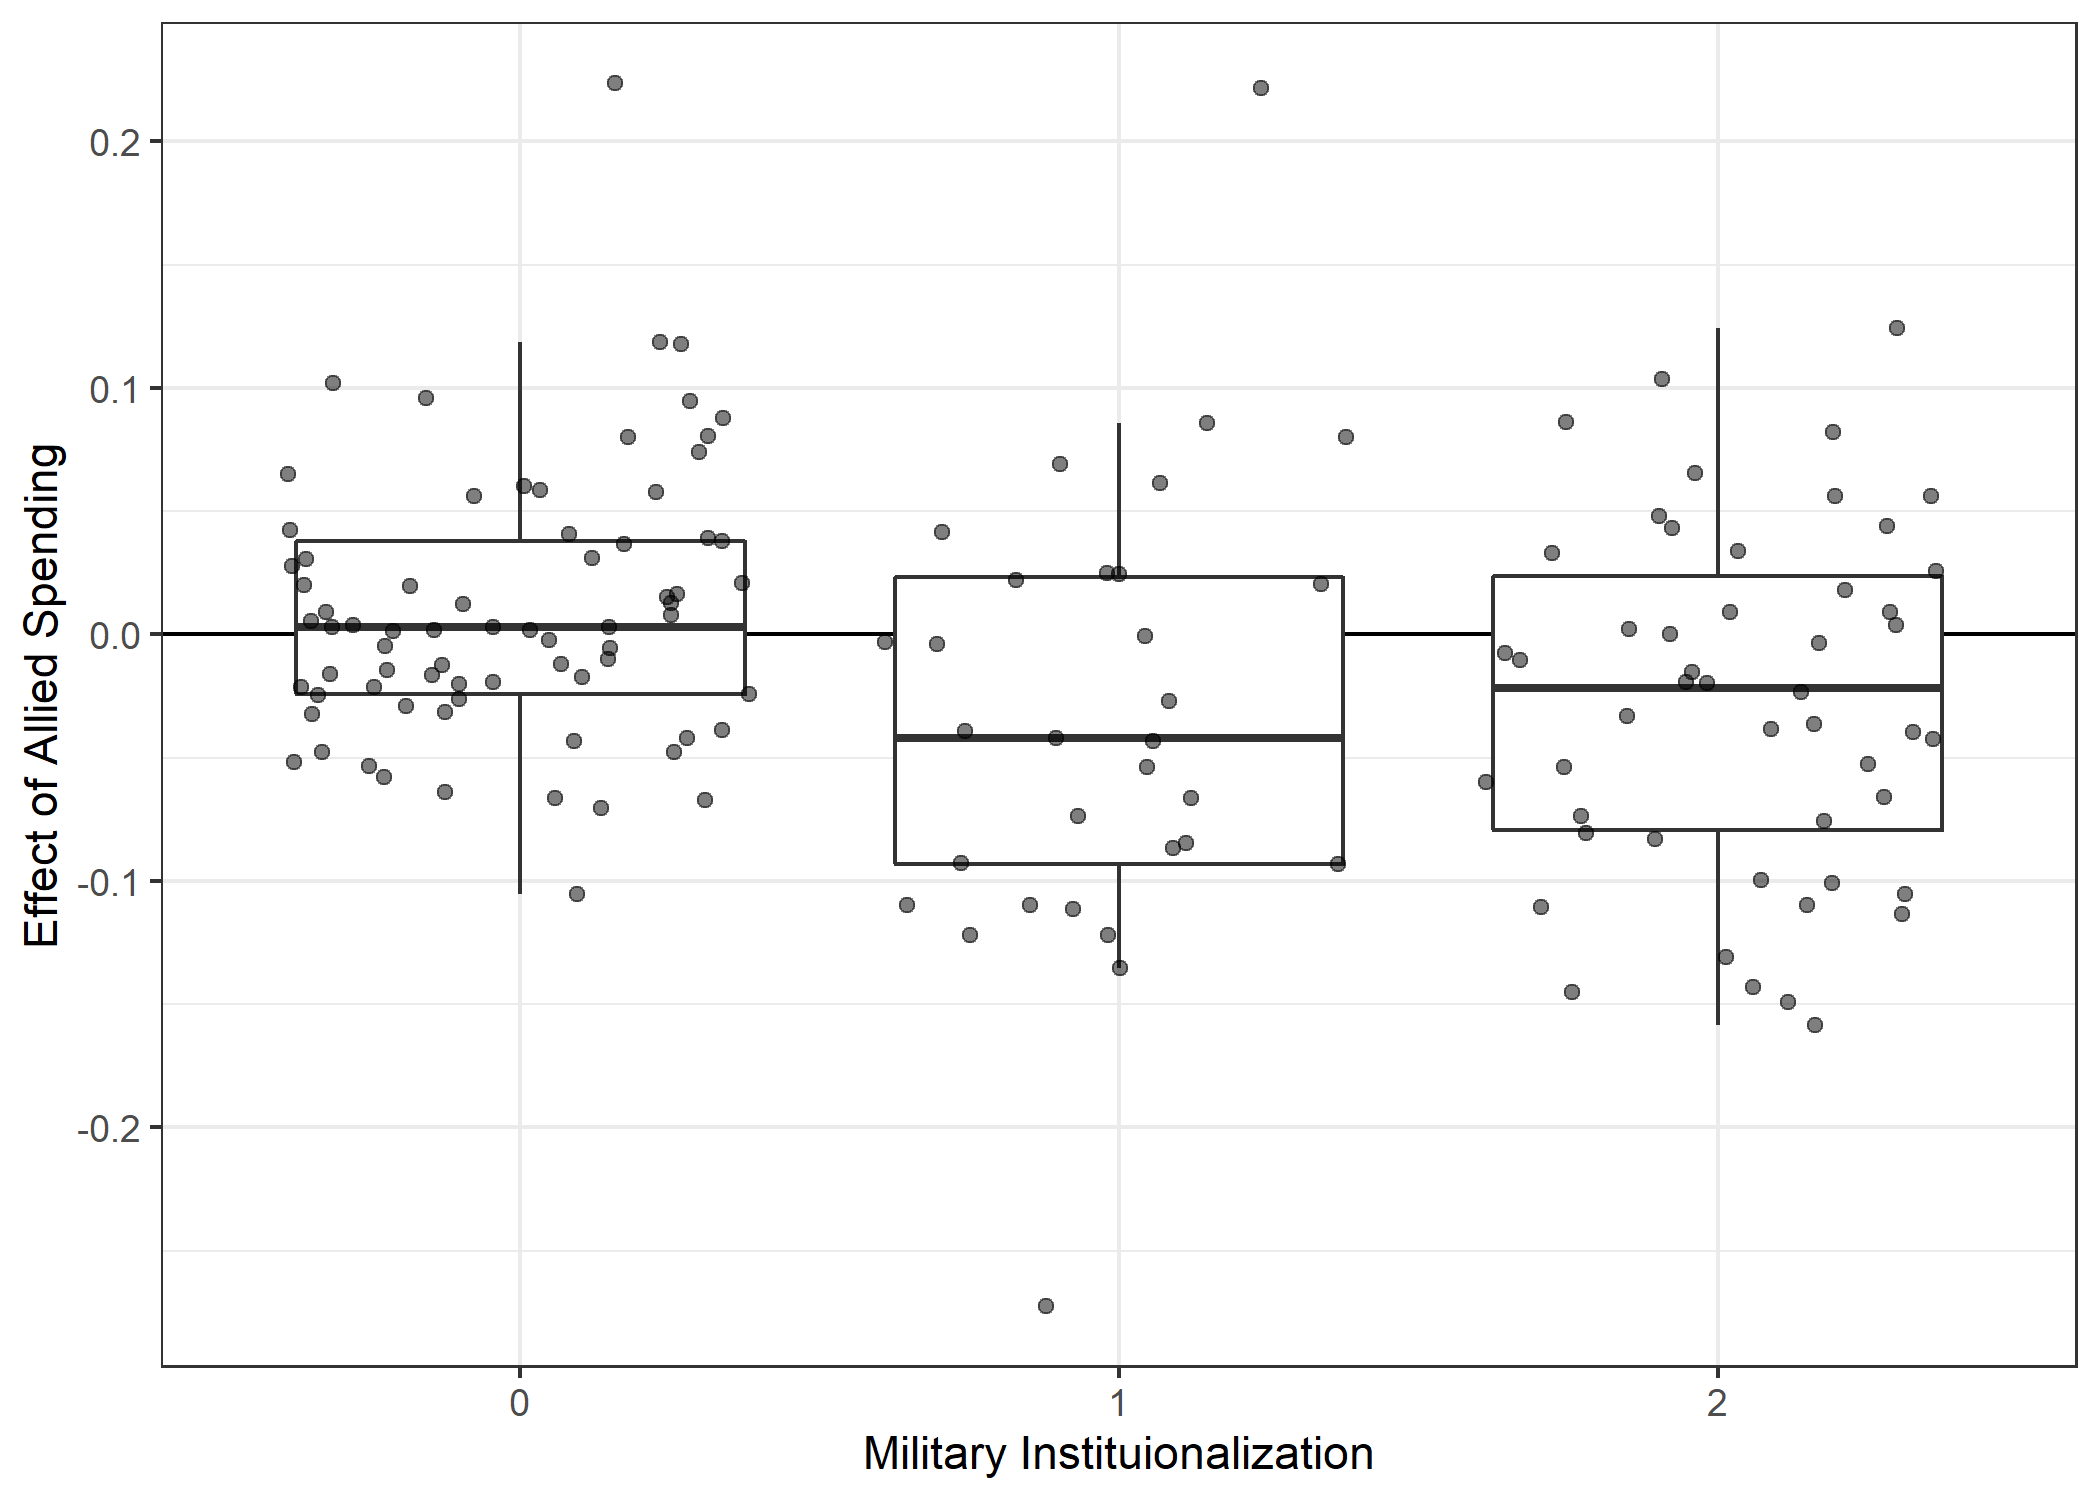
\includegraphics[width=0.95\textwidth]{milinst-lambda.png}
	\caption{Scatter plot of $\lambda$ parameters against the values of military institutionalization. The box plots summarize the distribution of points within in each military institutionalization value. All points are jittered to make the plot more legible.}
	\label{fig:milinst-lambda}
\end{figure}



\subsection{Benson and Clinton 2016}

Having established that an ordinal measure of treaty depth produces similar results, I now explain why I did not use an existing latent measure of treaty depth. 
\citet{BensonClinton2016} use a latent variable model to estimate alliance scope, depth and capability. 
I do not use their measure of depth because it captures a different concept, and thus diverges from my aims in this project. 
Benson and Clinton define depth as the general costliness of alliance obligations, which leads them to include other variables and measure the depth of neutrality pacts. 
I define depth in terms of military coordination and cooperation and am only interested in alliances with active military support. 
My focus on defensive and offensive alliances follows existing scholarship on alliance participation and military spending.
These conceptual differences, along with my use of a different estimator, lead to different conclusions about the factor loadings and the latent depth scores.


% including neutrality pacts changes the comparison category in the measurement model, essentially
Benson and Clinton aim for a broad measure of alliances, so they include neutrality pacts in their data. 
There is an understandable choice, but it means their measure diverges from the my argument, which focuses on alliances with military support. 
Neutrality pacts are qualitatively different, because peacetime coordination is not focused on ensuring the delivery of military support. 


In Benson and Clinton's measure, neutrality pacts have very little depth, which is unsurprising.
Neutrality is less costly in general.  
Only a few alliances with only neutrality obligations have any depth, as \autoref{fig:bc2016-neutral} shows.  


\begin{figure}[htbp]
	\centering
		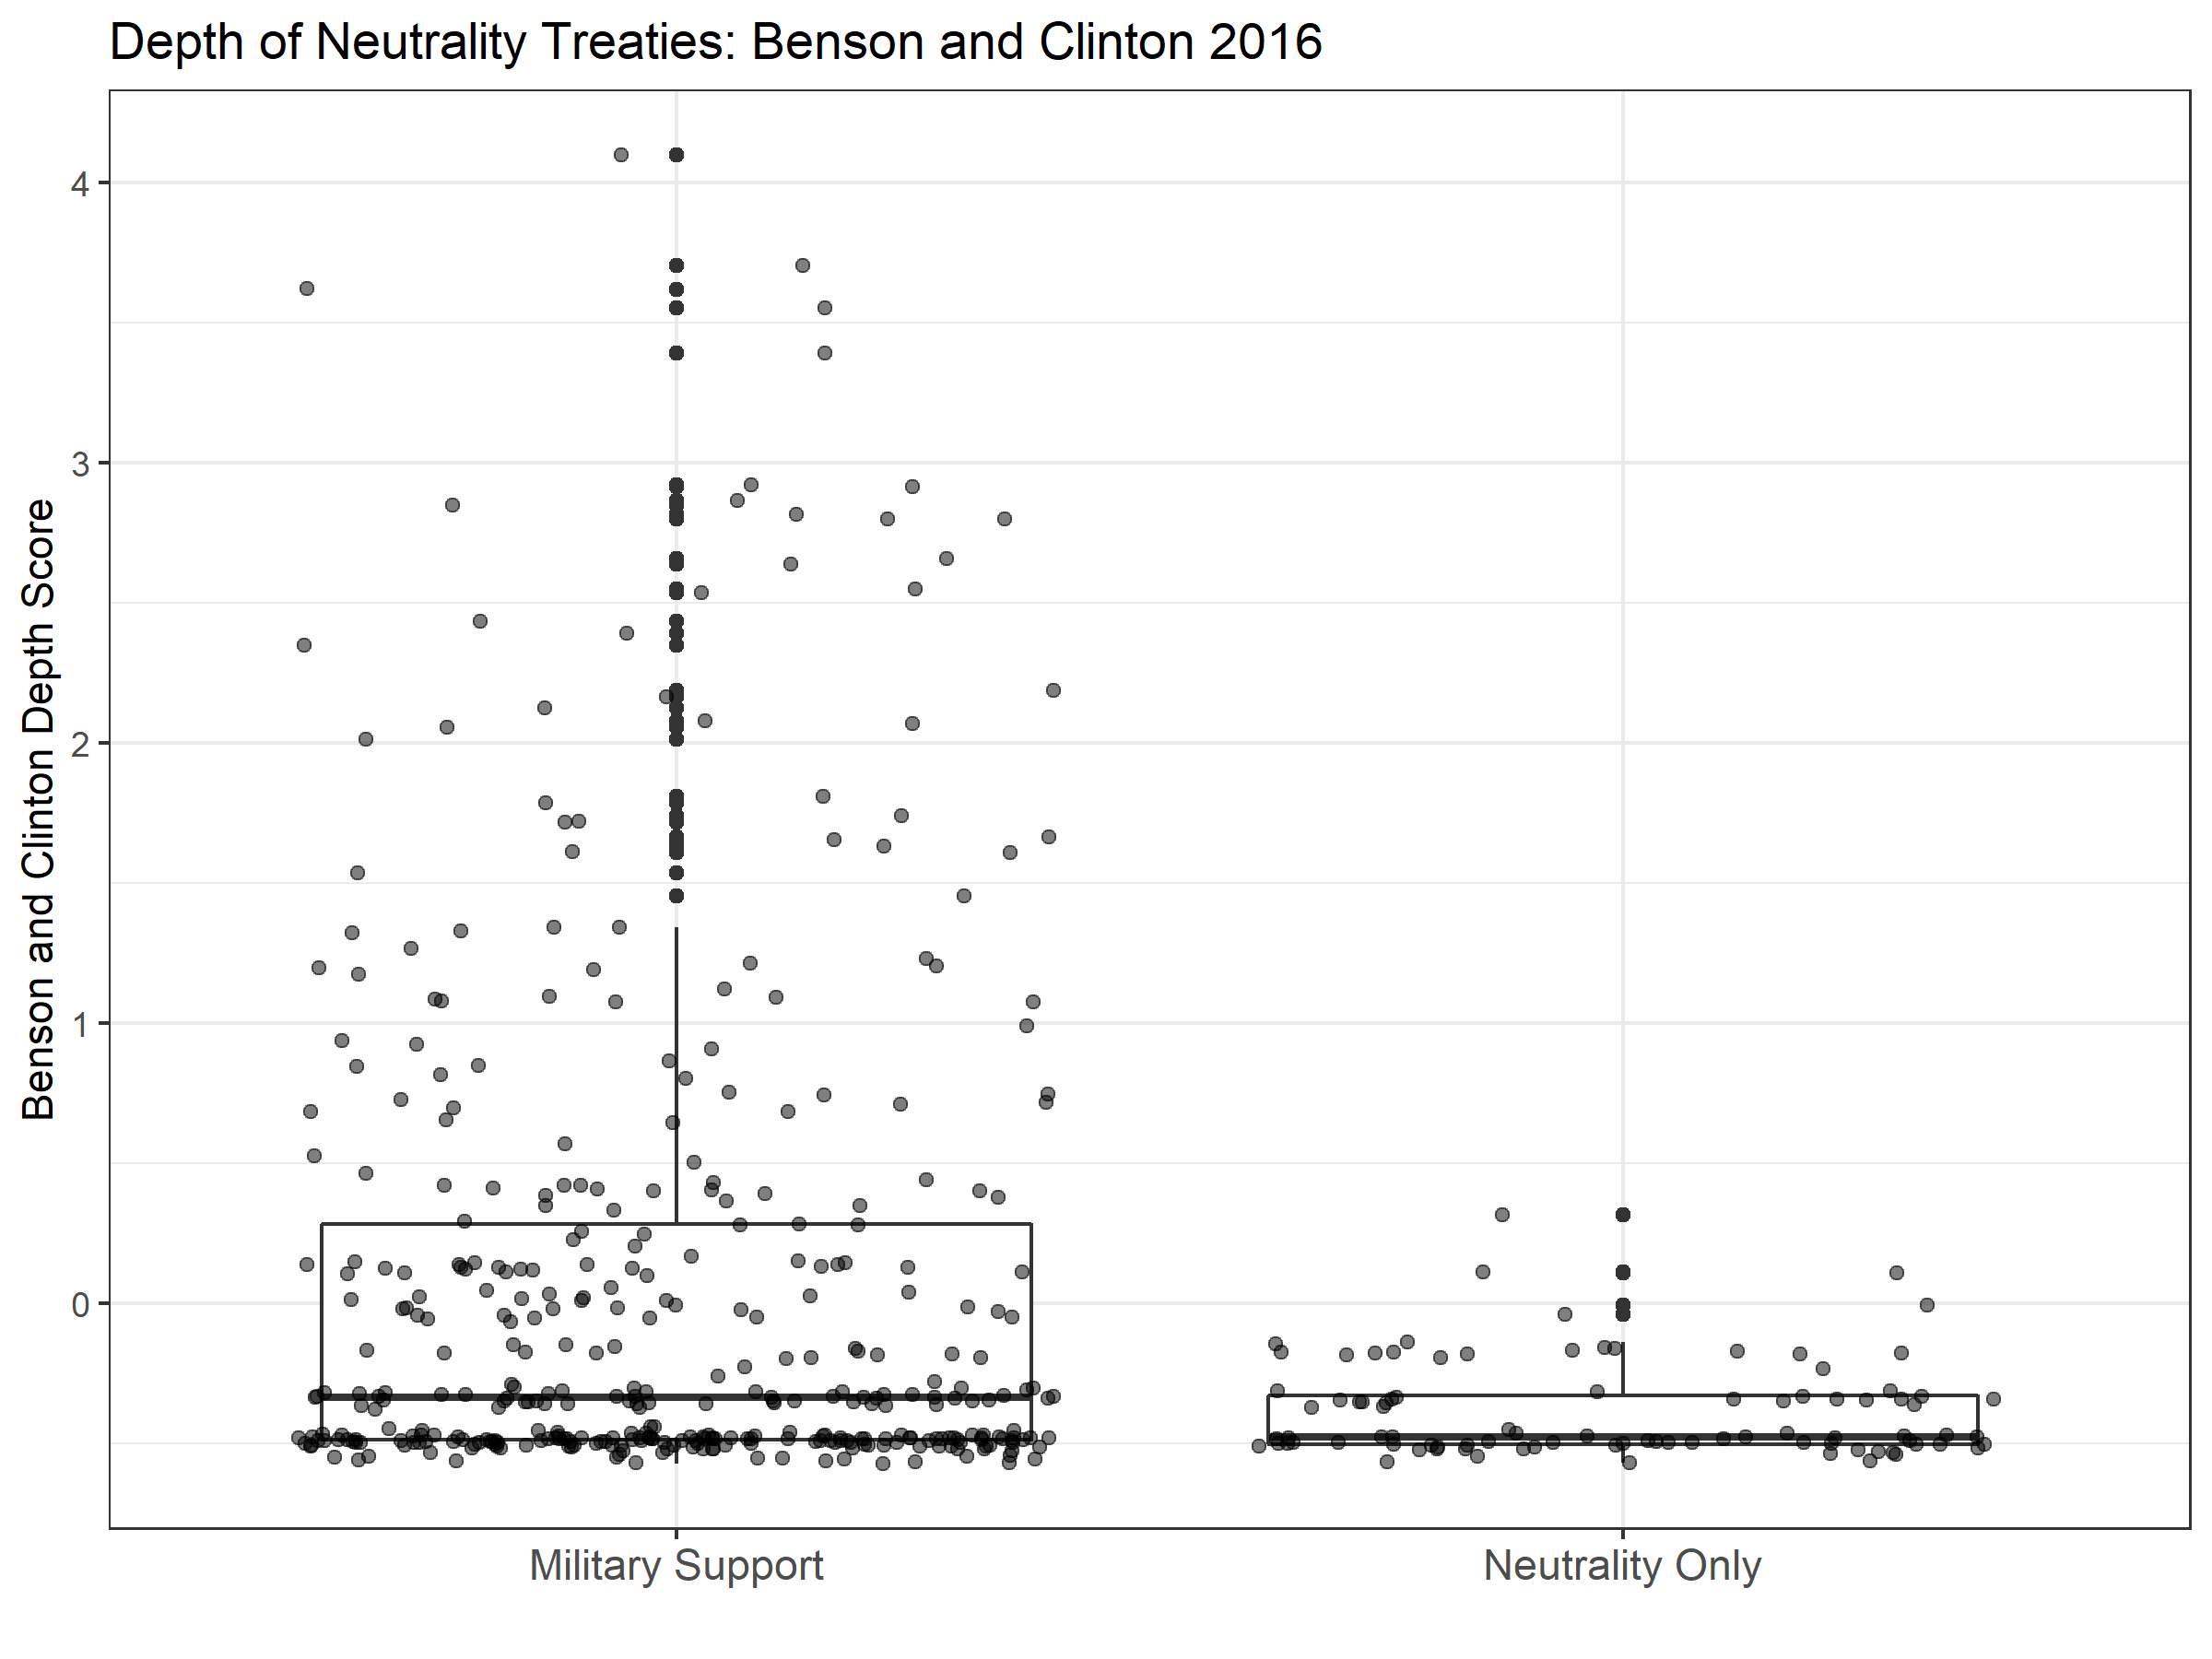
\includegraphics[width=0.95\textwidth]{bc2016-neutral.png}
	\caption{Comparison of Benson and Clinton's depth measure among alliances with only neutrality obligations and alliances with active offensive or defensive support. The box plots summarize the distribution of alliance depth within each group of alliances. All points are jittered to make the plot more legible.}
	\label{fig:bc2016-neutral}
\end{figure}
In estimation, neutrality pacts are something like a reference category for military alliances. 
Neutrality pacts have limited depth, but they inform inferences about the depth of alliances with offensive or defensive promises. 
By including neutrality pacts, Benson and Clinton's model compares alliances with generally limited obligations to alliances with active military support.


Again, Benson and Clinton's decision to measure the depth of neutrality pacts is not a problem for their paper. 
It limits the applicability of their measure to this project, however. 
I do not address neutrality pacts in my argument, so my measure of depth only considers variation among offensive and defensive alliances. 
My theoretical focus on military cooperation also leads me to exclude indicators of secrecy and economic aid that Benson and Clinton use to predict treaty depth. 
Although Benson and Clinton's measure is close to my purposes, it captures a slightly different concept. 


% differences in loadings and estimator have important consequences for depth scores
Given conceptuial differences and my decision to use a semiparametric estimator that breaks problematic correlations between the latent variables and dependence structure \citep{Murrayetal2013}, I draw different conclusions about the factor loadings and distribution of treaty depth. 
\autoref{fig:bc-2016-comp} describes the key differences between my latent measure of depth and Benson and Clinton's measure.
In the top panel, I look at differences in the factor loadings across the two models.\footnote{Recall that I removed economic aid and secrecy from the observed data in my measure, because they are distinct from military cooperation.} 
Benson and Clinton break the ATOP policy coordination variable into military contact and common defense policy, but I treat this as an ordinal variable, which is the largest source of depth.\footnote{The military contact variable on which the policy coordination score is based gives alliances that require wartime military contact a score of one, scores treaties with peacetime military contact as a two, and assigns alliances with defense cooperation a score of three. There is a order to the extent of policy coordination required as this variable increases.}
I also find larger correlations between formal organization and integrated military command and latent depth than Benson and Clinton.
It is harder to distinguish between the other loadings, but Benson and Clinton's measure assigns marginally more weight to military aid and basing rights.  


\begin{figure}[htbp]
	\centering
		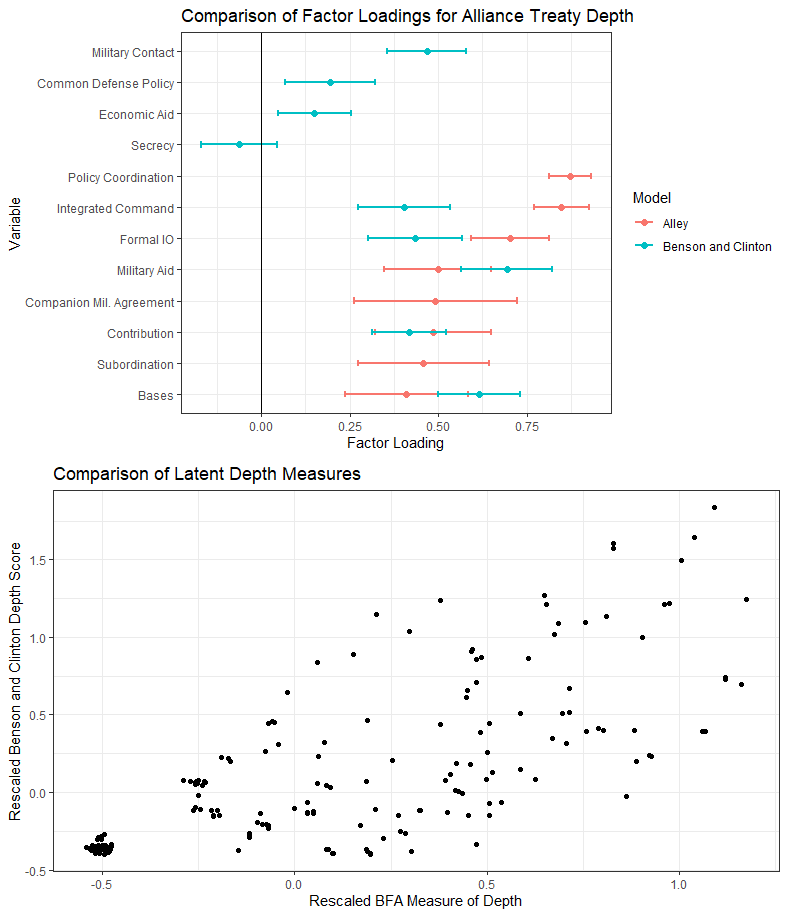
\includegraphics[width=0.95\textwidth]{bc-2016-comp.png}
	\caption{Comparison of latent measures of alliance treaty depth, one from this paper, and the other from \citet{BensonClinton2016}. The top panel compares the factor loadings from the two variables. The scatter plot compares latent depth scores from the semiparametric factor analysis with depth scores from \citet{BensonClinton2016}. The two latent measures have been rescaled by one standard deviation to facilitate comparisons. This comparison only includes alliances from version 3 of the ATOP data, because these are the alliances for which both models have scores.}
	\label{fig:bc-2016-comp}
\end{figure}


In the bottom panel of \autoref{fig:bc-2016-comp}, I plot my measure of treaty depth against Benson and Clinton's. 
To facilitate this comparison, I rescaled both depth measures by dividing them by one standard deviation.
Benson and Clinton's measure suggests 18 alliances are 2 or more standard deviations from the mean, while my measure contains 9 such alliances. 
Many treaties with high depth on Benson and Clinton's measure have lower depth relative to other alliances on my measure.
The two measures identify a common set of six extremely deep alliances, but disagree about how distinctive they are from other treaties. 
Salient distinctions in the relative depth of alliance treaties follow from differences in the factor loadings. 


Though the two measures of depth are correlated, they capture different concepts and my measure has fewer extreme outliers. 
Benson and Clinton address the general cost of an alliance, while I am focused on military coordination and cooperation. 
Benson and Clinton's measure is useful, but it departs from my aims in this project by including other variables and analyzing neutrality pacts. 
Because our measures operationalize different concepts in different groups of alliances, I believe my measure of depth is better suited for an analysis of the consequences of deep military cooperation in defensive and offensive alliances. 
My measure is not generally superior, and which latent depth measure scholars use in other analyses should depend on how they conceptualize alliance treaty depth. 



\section{Are Deep Alliances Less Reliable?} 


\citet{LeedsAnac2005} find that institutionalized alliances are less reliable, which contradicts my claim that deep alliances increase treaty reliability. 
Besides potential bias from non-random selection into challenges of alliances \citep{Smith1995}, this empirical finding depends in part on their ordinal institutionalization measure. 
Replacing the ordinal measure with my continuous latent depth variable leads to different inferences about alliance treaty design and performance. 
Therefore, the surprising finding in this paper that better institutionalized alliances have worse performance may also reflect measurement decisions. 


I focus my replication on Leeds and Anac's model of whether alliance members honor treaties with active military support. 
The replication focuses on this model because my argument examines defensive and offensive alliances. 
Their dataset includes 103 alliance performance opportunities, where states could honor or violate promises of military support. 
Using a logit model that adjusts for alliance formality, capability changes, changes in the policy process and whether the ally was the original target, Leeds and Anac find a negative relationship between institutionalization and performance. 
I replicate this estimate in the first column of \autoref{tab:depth-performance}. 


\begin{table}[!htbp] \centering 
\begin{adjustbox}{width= .95\textwidth, center}
\begin{tabular}{@{\extracolsep{5pt}}lcccccc} 
\\[-1.8ex]\hline 
\hline \\[-1.8ex] 
 & \multicolumn{6}{c}{\textit{Dependent variable:}} \\ 
\cline{2-7} 
\\[-1.8ex] & \multicolumn{4}{c}{Leeds and Anac} & \multicolumn{2}{c}{Berkemeier and Fuhrmann} \\ 
\\[-1.8ex] & \multicolumn{2}{c}{\textit{Logit}} & \multicolumn{2}{c}{\textit{Firth Logit}} & \textit{Logit} & \textit{Firth Logit} \\ 
\\[-1.8ex] & (1) & (2) & (3) & (4) & (5) & (6)\\ 
\hline \\[-1.8ex] 
 Military Institutionalization & $-$0.543 &  & $-$0.086 &  &  &  \\ 
  & ($-$1.306, 0.221) &  & ($-$0.190, 0.018) &  &  &  \\ 
  Latent Depth &  & 0.202 &  & 0.018 & 0.242 & 0.195 \\ 
  &  & ($-$0.527, 0.931) &  & ($-$0.090, 0.125) & ($-$0.443, 0.927) & ($-$0.450, 0.841) \\ 
  Alliance Formality & $-$1.161$^{}$ & $-$1.519$^{}$ & $-$0.169$^{}$ & $-$0.208$^{}$ &  &  \\ 
  & ($-$2.082, $-$0.240) & ($-$2.463, $-$0.575) & ($-$0.292, $-$0.046) & ($-$0.330, $-$0.087) &  &  \\ 
  Capability Change & $-$1.841$^{}$ & $-$1.931$^{}$ & $-$0.287$^{}$ & $-$0.293$^{}$ &  &  \\ 
  & ($-$3.135, $-$0.547) & ($-$3.256, $-$0.607) & ($-$0.480, $-$0.094) & ($-$0.489, $-$0.097) &  &  \\ 
  Process Change & $-$1.802$^{}$ & $-$1.462$^{}$ & $-$0.289$^{}$ & $-$0.243$^{}$ &  &  \\ 
  & ($-$3.336, $-$0.269) & ($-$2.886, $-$0.037) & ($-$0.519, $-$0.059) & ($-$0.471, $-$0.015) &  &  \\ 
  Original Target & $-$0.723 & $-$0.813 & $-$0.099 & $-$0.118 &  &  \\ 
  & ($-$1.849, 0.403) & ($-$1.979, 0.353) & ($-$0.273, 0.075) & ($-$0.300, 0.065) &  &  \\ 
  Asymmetric Capability &  &  &  &  & $-$1.791 & $-$1.450 \\ 
  &  &  &  &  & ($-$3.990, 0.407) & ($-$3.338, 0.438) \\ 
  Non-Major Only &  &  &  &  & $-$2.767$^{}$ & $-$2.251$^{}$ \\ 
  &  &  &  &  & ($-$5.120, $-$0.414) & ($-$4.303, $-$0.200) \\ 
  Post 1945 &  &  &  &  & $-$2.662$^{}$ & $-$2.339$^{}$ \\ 
  &  &  &  &  & ($-$4.134, $-$1.189) & ($-$3.690, $-$0.989) \\ 
  Average Democracy &  &  &  &  & 0.134$^{}$ & 0.117$^{}$ \\ 
  &  &  &  &  & (0.032, 0.235) & (0.021, 0.212) \\ 
  Number of Members &  &  &  &  & $-$0.228 & $-$0.120 \\ 
  &  &  &  &  & ($-$0.521, 0.064) & ($-$0.268, 0.027) \\ 
  Economic Issue Linkage &  &  &  &  & $-$0.451 & $-$0.386 \\ 
  &  &  &  &  & ($-$1.599, 0.698) & ($-$1.468, 0.697) \\ 
  Unconditional Support &  &  &  &  & 1.393 & 1.161 \\ 
  &  &  &  &  & ($-$0.331, 3.117) & ($-$0.383, 2.705) \\ 
  Foreign Policy Concessions &  &  &  &  & $-$0.247 & $-$0.239 \\ 
  &  &  &  &  & ($-$0.940, 0.447) & ($-$0.895, 0.417) \\ 
  Constant & 3.430$^{}$ & 3.162$^{}$ & 1.037$^{}$ & 0.987$^{}$ & 3.574$^{}$ & 2.812$^{}$ \\ 
  & (1.972, 4.888) & (1.780, 4.544) & (0.888, 1.186) & (0.849, 1.126) & (1.261, 5.887) & (0.895, 4.728) \\ 
 \hline \\[-1.8ex] 
Observations & 93 & 93 & 93 & 93 & 109 & 109 \\ 
Log Likelihood & $-$39.131 & $-$39.992 & $-$41.292 & $-$42.613 & $-$47.613 & $-$48.277 \\ 
\hline 
\hline \\[-1.8ex] 
\textit{Note:}  & \multicolumn{6}{r}{95\% Confidence Intervals in Parentheses.} \\ 
\end{tabular} 
\end{adjustbox} 
  \caption{Logit models of whether alliance members honored their treaty commitments in war.} 
  \label{tab:depth-performance}  
\end{table} 


I then replace Leeds and Anac's institutionalization measure with my latent treaty depth measure, which is in the second column of \autoref{tab:depth-performance}. 
The coefficient on depth, in contrast to military institutionalization, is positive, though neither estimate is statistically significant at conventional levels. 
Thus, the possible direction of this association shifts, depending on how alliance depth is measured.


To further assess this finding, I utilized an updated alliance performance dataset from \citet{BerkemeierFuhrmann2018}.
In this analysis, I specified a logit model that uses latent depth, unconditional support, dummy indicators of asymmetric capability or alliances only between non-major powers, a post 1945 dummy, the average polity score of alliance members when the treaty formed, the number of members, economic issue linkages, and foreign policy concessions to predict whether an alliance was honored in war. 
All of these factors are potential sources of reliability and correlates of depth. 


In both datasets, I employ standard logit and a firth logit estimator, because the sample is fairly small. 
Across all these models and estimators, I find a similar result--- a positive relationship between depth and honoring military support that cannot be distinguished from zero.
Therefore, I do not find that highly institutionalized alliances are less reliable. 
The change in the direction of the coefficient is suggestive, given the limited number of alliance performance opportunities in these datasets. 
Again, given non-random selection into alliance crises and challenges, placing excessive weight on the above results is unwise. 
They do suggest, however, that deep alliances are not necessarily less reliable when invoked. 





  
\bibliography{../../MasterBibliography} 




\end{document}
